\documentclass[sigconf,9pt,nonacm]{acmart}
\settopmatter{printfolios=true}
\renewcommand\footnotetextcopyrightpermission[1]{}
\setcopyright{none}
\pagestyle{plain}
\usepackage{booktabs,array}
\usepackage{xcolor}
\usepackage{xspace}
\usepackage{tikz}
\usetikzlibrary{arrows.meta}
% generated by make_assets_short.py - do not edit
\newcommand{\NCfg}{13}
\newcommand{\NExact}{12}
\newcommand{\NTcp}{14{,}200}
\newcommand{\NStageA}{5{,}200}
\newcommand{\NineShare}{35}
\newcommand{\NModelDiff}{25}
\newcommand{\NStageB}{9{,}000}
\newcommand{\CMaeZero}{0.30}
\newcommand{\CMaxZero}{0.7}
\newcommand{\CWrongZero}{0}
\newcommand{\CMaeOne}{7.39}
\newcommand{\CMaxOne}{99.4}
\newcommand{\CWrongOne}{2}
\newcommand{\CMaeTwo}{14.45}
\newcommand{\CMaxTwo}{99.4}
\newcommand{\CWrongTwo}{4}
\newcommand{\CMaeThree}{21.50}
\newcommand{\CMaxThree}{99.4}
\newcommand{\CWrongThree}{6}
\newcommand{\CN}{28}
\newcommand{\DN}{80}
\newcommand{\DDiff}{10}
\newcommand{\DJoinedWrongDiff}{10}
\newcommand{\DEarlyWrongDiff}{0}
\newcommand{\DJoinedMae}{17.8}
\newcommand{\DEarlyMae}{5.5}
\newcommand{\DJoinedWrong}{14}
\newcommand{\DEarlyWrong}{4}
\newcommand{\DBothWrong}{4}
\newcommand{\EFitEcdsa}{10}
\newcommand{\EFitMlFourFour}{12}
\newcommand{\EFitMlSixFive}{15}
\newcommand{\ECtlN}{36}
\newcommand{\ECtlMax}{0.9}
\newcommand{\ECtlWrong}{0}
\newcommand{\EN}{72}
\newcommand{\RJoinedMae}{1.42}
\newcommand{\RJoinedMax}{98.8}
\newcommand{\RJoinedWrong}{2}
\newcommand{\RJoinedRest}{142}
\newcommand{\RN}{144}
\newcommand{\RJoinedRestMax}{0.85}
\newcommand{\REarlyMae}{0.54}
\newcommand{\REarlyMax}{0.8}
\newcommand{\REarlyWrong}{0}
\newcommand{\REarlyRest}{144}
\newcommand{\RaceN}{221}
\newcommand{\RaceMlN}{134}
\newcommand{\RaceThr}{0.049}
\newcommand{\RaceRight}{132}
\newcommand{\RaceBeforePct}{90}
\newcommand{\RaceTwoRight}{36}
\newcommand{\RaceTwoScored}{36}
\newcommand{\RaceTwoOosRight}{394}
\newcommand{\RaceTwoOosN}{399}
\newcommand{\MixFitExc}{13}
\newcommand{\MixPredExc}{15}
\newcommand{\MixN}{4}
\newcommand{\MixRight}{3}
\newcommand{\NineDefMaeBefore}{13.3}
\newcommand{\NineDefMaeAfter}{1.2}
\newcommand{\NineN}{48}
\newcommand{\NineRwndDefOk}{7}
\newcommand{\NineRwndDefTot}{20}
\newcommand{\NineRwndLargeOk}{16}
\newcommand{\NineRwndLargeTot}{20}
\newcommand{\GenCells}{240}
\newcommand{\GenRespMax}{16}
\newcommand{\GenRttLo}{5}
\newcommand{\GenRttHi}{100}
\newcommand{\GenRateLo}{10}
\newcommand{\GenRateHi}{100}
\newcommand{\GenMtuLo}{1\,280}
\newcommand{\GenMtuHi}{9\,000}
\newcommand{\GenWEcRttFive}{10}
\newcommand{\GenWMFourFourRttFive}{10}
\newcommand{\GenWMSixFiveRttFive}{10}
\newcommand{\GenWEcRttThirty}{10}
\newcommand{\GenWMFourFourRttThirty}{12}
\newcommand{\GenWMSixFiveRttThirty}{15}
\newcommand{\GenWEcSlowTen}{10}
\newcommand{\GenWMFourFourSlowTen}{10}
\newcommand{\GenWMSixFiveSlowTen}{10}
\newcommand{\GenWEcMtuLow}{10}
\newcommand{\GenWMFourFourMtuLow}{12}
\newcommand{\GenWMSixFiveMtuLow}{16}
\newcommand{\ServCells}{48}
\newcommand{\ServWindow}{10}
\newcommand{\ServWrong}{0}
\newcommand{\BkN}{664}
\newcommand{\BkDef}{235}
\newcommand{\BkAOne}{44}
\newcommand{\BkAPct}{23.0}
\newcommand{\BkBRight}{248}
\newcommand{\BkBPct}{57.8}
\newcommand{\NtkRight}{18}
\newcommand{\NtkCells}{18}
\newcommand{\NtkEffect}{7}
\newcommand{\NtkEffectOk}{7}
\newcommand{\HN}{331}
\newcommand{\HLate}{117}
\newcommand{\HEarly}{214}
\newcommand{\HLateSS}{117}
\newcommand{\HWaitMed}{13.7}
\newcommand{\HEarlySS}{19}
\newcommand{\HAOne}{6}
\newcommand{\HALate}{117}
\newcommand{\HAPct}{5.1}
\newcommand{\HEnqMed}{181.2}
\newcommand{\HPcapMed}{-0.073}
\newcommand{\PhAfter}{164}
\newcommand{\PhAfterSS}{164}
\newcommand{\PhBefore}{500}
\newcommand{\PhBeforeSS}{61}
\newcommand{\StN}{799}
\newcommand{\StPOneRight}{799}
\newcommand{\StPOneN}{799}
\newcommand{\StPOnePct}{100.0}
\newcommand{\StPTwoRight}{212}
\newcommand{\StPTwoN}{236}
\newcommand{\StPTwoPct}{89.8}
\newcommand{\StPThreeRight}{51}
\newcommand{\StPThreeN}{74}
\newcommand{\StPThreePct}{68.9}
\newcommand{\StPTwoBRight}{236}
\newcommand{\StPTwoBN}{236}
\newcommand{\StDeferred}{71}
\newcommand{\StDeferredN}{96}
\newcommand{\StLate}{204}
\newcommand{\StLateInflight}{179}
\newcommand{\StLateLimited}{182}
\newcommand{\StEarly}{595}
\newcommand{\StEarlyLimited}{13}
\newcommand{\StBeforeN}{570}
\newcommand{\StBeforePk}{1}
\newcommand{\StAfterN}{204}
\newcommand{\StAfterPk}{10}
\newcommand{\KerN}{288}
\newcommand{\KerBeforeN}{216}
\newcommand{\KerBeforeSS}{0}
\newcommand{\KerAfterN}{72}
\newcommand{\KerAfterSS}{47}
\newcommand{\KerRight}{274}
\newcommand{\KerPct}{95.1}
\newcommand{\KerWrong}{14}
\newcommand{\KerMissLo}{0.039}
\newcommand{\KerMissHi}{0.080}
\newcommand{\KerMissNear}{0.031}
\newcommand{\AblFixedMae}{2.30}
\newcommand{\AblFixedOff}{4}
\newcommand{\AblFixedN}{144}
\newcommand{\AblSlowMae}{1.42}
\newcommand{\AblSlowOff}{2}
\newcommand{\AblSlowN}{144}
\newcommand{\AblLinuxMae}{1.42}
\newcommand{\AblLinuxOff}{2}
\newcommand{\AblLinuxN}{144}
\newcommand{\AblJoinedMae}{1.42}
\newcommand{\AblJoinedOff}{2}
\newcommand{\AblJoinedN}{144}
\newcommand{\AblEarlyMae}{0.54}
\newcommand{\AblEarlyOff}{0}
\newcommand{\AblEarlyN}{144}
\newcommand{\AblCFixedMae}{25.04}
\newcommand{\AblCFixedOff}{7}
\newcommand{\AblCFixedN}{28}
\newcommand{\AblCSlowMae}{35.63}
\newcommand{\AblCSlowOff}{10}
\newcommand{\AblCSlowN}{28}
\newcommand{\AblCLinuxMae}{0.30}
\newcommand{\AblCLinuxOff}{0}
\newcommand{\AblCLinuxN}{28}
\newcommand{\OvTwoSame}{247}
\newcommand{\OvTwoAll}{252}
\newcommand{\OvThreeSame}{247}
\newcommand{\OvThreeAll}{252}
\newcommand{\OvFourSame}{236}
\newcommand{\OvFourAll}{252}
\newcommand{\GxBaseCWrong}{0}
\newcommand{\GxBaseCLoose}{4}
\newcommand{\GxBaseDisEarly}{0}
\newcommand{\GxBaseDisJoined}{10}
\newcommand{\GxBaseEarlyWrong}{4}
\newcommand{\GxBaseMet}{4}
\newcommand{\GxFourCWrong}{0}
\newcommand{\GxFourCLoose}{4}
\newcommand{\GxFourDisEarly}{0}
\newcommand{\GxFourDisJoined}{10}
\newcommand{\GxFourEarlyWrong}{4}
\newcommand{\GxFourMet}{4}
\newcommand{\GxThreeCWrong}{0}
\newcommand{\GxThreeCLoose}{4}
\newcommand{\GxThreeDisEarly}{0}
\newcommand{\GxThreeDisJoined}{10}
\newcommand{\GxThreeEarlyWrong}{4}
\newcommand{\GxThreeMet}{4}
\newcommand{\GxMaxDiff}{0.05}
\newcommand{\CiWinLo}{64.0}
\newcommand{\CiWinHi}{99.8}
\newcommand{\CiJoinedLo}{95.1}
\newcommand{\CiJoinedHi}{99.8}
\newcommand{\CiRaceLo}{94.7}
\newcommand{\CiRaceHi}{99.8}
\newcommand{\CiKerLo}{92.0}
\newcommand{\CiKerHi}{97.3}
\newcommand{\CiNtkEffLo}{59.0}
\newcommand{\CiNtkEffHi}{100.0}
\newcommand{\SignDP}{0.002}
\newcommand{\SignNtkP}{0.016}

\newcommand{\pending}[1]{{\color{red}\textit{[pending: #1]}}}
\newcommand{\ms}{\,ms\xspace}
\newcommand{\citeone}{\cite{paperone}}
\graphicspath{{../Latex/figures/}}
\hyphenation{OpenSSL ac-knowl-edg-ment}
\setlength{\emergencystretch}{2em}

\begin{document}
\title{How Linux Grows the TCP Window After a Short Flight, and What It Costs Post-Quantum TLS in Round Trips}
\author{Trong-Hieu Dinh}
\affiliation{\institution{Banking Academy of Vietnam}\city{Hanoi}\country{Vietnam}}
\email{hieudt@hvnh.edu.vn}
\author{Trong-Minh Hoang}
\authornote{Corresponding author.}
\affiliation{\institution{Posts and Telecommunications Institute of Technology}\city{Hanoi}\country{Vietnam}}
\email{hoangtrongminh@ptit.edu.vn}
\begin{abstract}
Post-quantum signatures push TLS flights past TCP's initial ten-segment window, so Linux's window growth affects round trips. A one-line rule is exact in \NExact\ of \NCfg\ plain-TCP configurations: five segments leave the window at ten, six at twelve. Predictions fixed in advance refute a larger client window and point to OpenSSL's separately written session ticket behind a latency-model error; without it, server bursts stay within ten segments. Once ACK processing times are known, the server's window follows slow start; predicting them remains open. The rule fails under BBR. The model overestimated latency in five of 100 random cells.
\end{abstract}
\begin{CCSXML}
<ccs2012>
<concept><concept_id>10003033.10003039.10003048</concept_id><concept_desc>Networks~Transport protocols</concept_desc><concept_significance>500</concept_significance></concept>
<concept><concept_id>10003033.10003079.10011704</concept_id><concept_desc>Networks~Network measurement</concept_desc><concept_significance>300</concept_significance></concept>
<concept><concept_id>10002978.10003014.10003015</concept_id><concept_desc>Security and privacy~Security protocols</concept_desc><concept_significance>300</concept_significance></concept>
</ccs2012>
\end{CCSXML}
\ccsdesc[500]{Networks~Transport protocols}
\ccsdesc[300]{Networks~Network measurement}
\makeatletter\g@addto@macro\@concepts{\linebreak}\makeatother % break before the second bullet of the CCS concepts
\ccsdesc[300]{Security and privacy~Security protocols}
\keywords{TLS 1.3, post-quantum cryptography, TCP congestion window, measurement, design guidance}
\maketitle

\section{Introduction}
Post-quantum signatures are big: 3\,309 bytes for ML-DSA-65 against about 70 for ECDSA-P256, nearly fifty times as many. A certificate chain that carries them no longer fits in Linux's 10-segment initial window~\cite{rfc6928}, and a flight that overflows the window can cost a round trip. Dukkipati et al.\ argued for that window from web latency~\cite{dukkipati2010}, and R\"uth et al.\ measured it across the IPv4 address space~\cite{rueth2017}. Both look at the window a connection starts with. We look at what happens next. How far the kernel grows the window after a short flight decides whether the following one (a request that carries a client certificate, say) fits in it, and so does the way the TLS library splits its data into writes.

Post-quantum handshakes are known to be slower~\cite{paquin2020,sikeridis2020,sosnowski2023,kampanakis2024}, but the closest studies treat the window as a setting. Henrich et al.\ vary the initial window in an emulated study of key-exchange algorithms: handshake times rise in steps once the data exceed it, and a larger window removes the extra round trips~\cite{henrich2025}. Chou and Cao see the time to first byte climb in steps as certificate chains cross the initial window, but approximate later windows by doubling, and process startup may mask their resumption times~\cite{chou2026}. Anastasova and Kampanakis attribute an increase of 51\ms (33\%) at 50\ms RTT to a client chain larger than the client's initial window (10 segments, against 24 on the server); they do not study resumption~\cite{anastasova2025}. A recent systems study counts the server's TCP segments in full handshakes (five connections per condition) and examines the loss tail; it tracks neither window growth between flights nor resumed connections~\cite{dubetskyy2026}. We found no direct measurement of the window after short flights in this setting.

How the window grows is trickier than it looks. RFC~5681 specifies slow start, RFC~2861 and its successor RFC~7661 specify congestion window validation~\cite{rfc5681,rfc2861,rfc7661}, and Linux lets the window grow in slow start up to twice the largest number of packets in flight~\cite{linuxcwnd}. Does a five-segment flight pass the test $10<2\times5$? That single inequality can decide a round trip. Our interest grew out of a failure. A per-segment transport model (Section~\ref{sec:method}), first built for full handshakes~\citeone, was right to within 1\ms\ on \RJoinedRest\ of \RN\ resumed OpenSSL~3.5 configurations (exact 95\% interval \CiJoinedLo--\CiJoinedHi\%; largest error \RJoinedRestMax\ms) and wrong by a whole round trip on two, both ML-DSA-44 with a large request (99\ms at 100\ms RTT, 29\ms at 30\ms): those transactions took one round trip fewer than the model predicted.

We ask three questions. \emph{RQ1:} how far does Linux grow the window after a short flight? \emph{RQ2:} why did the model predict a round trip that those two transactions never needed? \emph{RQ3:} what sets the server's window after the session ticket, and how well can it be predicted?

We make four contributions. (1)~For RQ1, a closed-form rule derived from the kernel's window validation: it is exact in \NExact\ of \NCfg\ configurations on one machine, four of which we repeat on \NCombW\ machine-kernel combinations, and we test it under packet loss (Section~\ref{sec:window}). (2)~For RQ2, tests with predictions fixed in advance that refute a larger client window and support a different cause, a session ticket that OpenSSL writes separately (Section~\ref{sec:ticket}). (3)~For RQ3, interventions. Removing the ticket removes the enlargement of the server's window, and kernel counters read at every ACK, while we delay the ACKs or the server's write, show that window and burst follow the slow-start rule once the ACK processing times are known (Section~\ref{sec:server}). (4)~Replications across kernels, CPUs, TLS libraries, BBR, a physical link, load, and random cells, and five recommendations (Sections~\ref{sec:repl}--\ref{sec:recs}). The rule's ingredients are in the RFCs and the kernel; new is measuring where they leave the window and what a TLS library's writes do with it. Unmet registered criteria are reported as such, here or in the supplement.

\section{Method}\label{sec:method}
The testbed consists of two network namespaces joined by a virtual Ethernet (veth) pair and shaped with \texttt{tc netem}. We call our machines \emph{X250} (Lenovo ThinkPad X250, i7-5600U) and \emph{OptiPlex} (Dell OptiPlex 7460, i7-8700), \emph{i9} (a workstation with an Intel i9-10900K), all x86-64, and \emph{GX10} (ASUS Ascent GX10, Arm Cortex-X925 and A725); the GX10 and the i9 are shared laboratory machines. The main platform is the X250 (Linux 7.0.0-42, OpenSSL~3.5); Section~\ref{sec:repl} repeats tests elsewhere. The CPU clock is fixed (performance governor, no turbo). TCP runs over IPv6 without timestamps (MSS = MTU$-60$) and with Reno. Unless stated otherwise, ACKs are sent immediately (\texttt{quickack} routes). ``Window'' means the sender's congestion window (\texttt{snd\_cwnd}, in segments); the receiver's advertised window is always called the ``receive window.'' A \emph{session ticket} travels in the NewSessionTicket message, which lets the client resume the session later. OpenSSL's server writes it when the client's Finished arrives, and under mutual authentication it contains the client certificate. The server's \emph{burst} is the number of response segments it sends before the first ACK of the response can return, that is, the window it actually used.

\emph{Plain TCP.} Each measurement opens a new connection and writes $n_1$ full-sized segments. Once a 100-byte reply has acknowledged them all, we read the window from \texttt{TCP\_INFO}. After an 80-byte write that stands in for a TLS Finished, we send a second flight of $n_2$ segments and time it. Stage~A reads the window after $n_1=\NOneList$ in \NCfg\ configurations that change one factor at a time: RTT 5--100\ms; 10\,Mbit/s--1\,Gbit/s; MTU 1\,280, 1\,500, 9\,000; initial window 4, 10, 20; delayed ACK; Cubic; timestamps; offload (\NStageA\ connections). Stage~B times the second flight in six configurations (\NStageB\ connections).

\emph{The model.} We predict latency by replaying each transaction deterministically, segment by segment (\texttt{Simulation/pqc\_sim.py}). A resumed transaction is a TCP handshake and four flights: ClientHello; the server's flight up to its Finished; the client's Finished and request; and the response, with a new ticket. Message sizes are calibrated on OpenSSL~3.5, and each flight is segmented in the order of its \texttt{write} calls. A sender starts a flight with its current window; the link is first-in, first-out with the given rate and RTT, and each ACK, sent immediately, releases up to two more segments. Each direction starts with a window of 10 and carries it to its next flight after growing it ACK by ACK under the kernel's window test (Section~\ref{sec:window}). This replay departs from rule~(1) only for odd $n\ge 11$, and in our resumed OpenSSL transactions no flight that precedes another in the same direction is that long. The model has two variants, which differ in where they put the ticket. The \emph{joined-ticket} model writes it with the response. The \emph{early-ticket} model writes it separately when the client's Finished arrives. If the request flight then needs another round trip, the ticket is acknowledged before the response is sent and takes no room in the response's window; otherwise the two share that window. Neither variant lets the response start with a window larger than ten segments. The model omits loss, delayed ACKs, pacing, the receive window, and congestion avoidance, and no parameter is fitted to a latency. It also omits cryptographic processing, so we compare its output with the measured \emph{excess latency}: the median on the shaped link minus the median on the unshaped link for the same suite and chain depth. A prediction is wrong if it is off by more than half an RTT. A \emph{discriminating} cell is one where the predictions of two models differ by more than that.

\emph{TLS with fixed predictions.} The TLS tests use resumed TLS~1.3 with mutual authentication, RTT 100\ms and \NPerCell\ transactions per cell. With four signature algorithms (ECDSA-P256, ML-DSA-44, -65, and -87), ClientHellos span \ChSegEc, \ChSegMlFourFour, \ChSegMlSixFive, and \ChSegMlEightSeven\ segments, because a resuming ClientHello carries the ticket and, with it, the client certificate. Before each measurement we committed the predictions of every compared rule or model for every cell. Table~\ref{tab:tests} lists 31 rows of tests and their outcomes; further tests (a third TLS library, a second random draw, and four rounds of an intervention) are reported in the supplement, and the appendix says how to repeat the key results. Rows 1--5 count cells that are wrong by a round trip. Rows 1 and 4, the rules we propose, were allowed none; rows 2 and 3 are alternatives that the tests set out to refute; and row 5 is a count without a criterion. Other rows report results against registered criteria (thresholds in the supplement). The archive lists, with checksums, the commit times of the predictions and of the first results (\texttt{PREREGISTRATION\_L1.md}). These are git timestamps, not independent ones; for the kernel and state traces only the analysis scripts and their thresholds were committed before the run. Within a ticket-timing or client-window cell, latency varies far less than one RTT (median interquartile range \SpreadMed\ms, maximum \SpreadMax\ms).

\section{The Window After a Short Flight}\label{sec:window}
The window after an $n$-segment flight is
\begin{equation}
w(n)=\max\bigl(w_0,\;\min(w_0+n,\;2n)\bigr),
\end{equation}
which holds exactly in \NExact\ of \NCfg\ configurations (exact 95\% interval \CiWinLo--\CiWinHi\%). The configurations differ in one factor each, so they are not independent and the interval is only descriptive. In words: up to $n=w_0/2$ the window does not grow; between $w_0/2$ and $w_0$ it is $2n$; from $w_0$ on, every segment of the flight adds one. Figure~\ref{fig:window} plots medians of 20 connections against (1) and its bounds $2n$ and $w_0+n$ (dotted).

Three kernel functions produce this behavior (mainline, checked November 18, 2026). With one ACK per segment, \texttt{tcp\_\allowbreak reno\_\allowbreak cong\_\allowbreak avoid} returns at once unless \texttt{tcp\_\allowbreak is\_\allowbreak cwnd\_\allowbreak limited} holds; only then does \texttt{tcp\_\allowbreak slow\_\allowbreak start} add the newly acknowledged segments to the window. The test holds if the sender was cwnd-limited when it sent (flag \texttt{is\_\allowbreak cwnd\_\allowbreak limited}, set by \texttt{tcp\_\allowbreak cwnd\_\allowbreak validate} when a flight fills the window) or, in slow start, while $\texttt{snd\_\allowbreak cwnd}<2\,\texttt{max\_\allowbreak packets\_\allowbreak out}$, where the right-hand side is twice the largest number of segments in flight, not twice the window. A flight of $n\ge w_0$ segments fills the window, so each of its $n$ ACKs adds one segment and the window ends at $w_0+n$. A shorter flight leaves the window unfilled, with $n$ segments in flight: the window grows by one per ACK until it reaches $2n$, and not at all if $w_0\ge 2n$.

A short program that implements this logic reproduces (1) for all \KernPairs\ pairs of $w_0\in\{2,4,10,16,20,32\}$ and $n\le 80$, and it matches the measured window at every point of the stage~A scan except at MTU 9\,000 (\texttt{Simulation/window\_\allowbreak from\_\allowbreak kernel.py}). At MTU~9\,000, the one configuration where (1) fails, only \NineShare\% of the flight sizes match, and the same logic explains why. The default receive buffer allows only about seven segments of 8\,940 bytes in flight, so the receive window stops the sender before the congestion window does; \texttt{is\_\allowbreak cwnd\_\allowbreak limited} stays false, and the window does not grow. With \texttt{tcp\_rmem} raised to 1\,MiB, \NineRwndLargeOk\ of \NineRwndLargeTot\ flight sizes follow (1), compared with \NineRwndDefOk\ by default. The remaining \NineFailNW\ (\NineFailLo\ to \NineFailHi\ segments) end one or two segments below it, which we cannot explain.

For TLS, what counts is the threshold. With $w_0=10$, $w(5)=\WFive$ and $w(6)=\WSix$: a five-segment ClientHello leaves the window unchanged, and a six-segment one raises it. In stage~B, once the model is given the window the kernel actually used, it predicts the completion time of the second flight with a mean error of \StageBLo--\StageBHi\ms.

\emph{Loss.} We also dropped 0.1, 0.5, and 1\% of the packets independently in each direction (stage~A, \GsixConn\ connections on each of the X250 and the i9; row 19 of Table~\ref{tab:tests}). Without a retransmission the rule almost always holds: \GsixNoRetxOk\ of \GsixNoRetxN\ such connections on the X250 (\GsixNoRetxPct\%) and \GsixINoRetxOk\ of \GsixINoRetxN\ on the i9 (\GsixINoRetxPct\%) end with the window of (1). Retransmissions become common as loss and flight size grow, reaching \GsixWorstRetx\% of connections at 1\% loss and 40 segments on the X250. We had predicted that the share of connections ending with the window of (1) would be $(1-p)^n$ for loss rate $p$, as if any lost packet broke the rule. The criterion, at least 24 of the \GsixCells\ cells within six points of that prediction, was missed on the X250 (\GsixWithin\ were) and only just met on the i9 (\GsixIWithin). In every cell off by more than six points, on both machines, the rule holds more often than predicted (\GsixWorstMeas\% against \GsixWorstPred\% at 1\% loss and 40 segments on the X250).

\begin{figure}[t]
\centering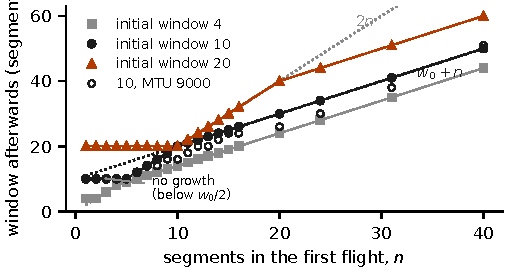
\includegraphics[width=\columnwidth]{fig_window_v3}
\caption{Window after an $n$-segment flight on plain TCP.}
\label{fig:window}
\end{figure}

\section{Why the Model Predicted Too Much: The Ticket}\label{sec:ticket}
\emph{A larger client window?} Take ML-DSA-44 with a \CellReq-byte request. The ClientHello is \ChSegMlFourFourW\ segments, so the window stays at 10 and the \CellReqSegsW-segment request flight costs a round trip. The model also put the ticket (about \NstKBMlFourFour\,KB) in the response flight, which then has \CellRespSegsW\ segments and costs a second round trip. The transaction needed only one of the two (\ExMeasMlFourFour\ms measured, \ExJoinedMlFourFour\ms predicted, at 100\ms RTT). Loosening the rule by two segments, chosen after seeing the data, removes the first and lowers the mean error over the \RN\ configurations to about \LooseMae\ms, but a test with predictions fixed in advance refutes it (Table~\ref{tab:tests}). Its \CN\ cells combine request flights of 9--15 segments with a 222-byte response, so that only the client's flight can cost an extra round trip (Fig.~\ref{fig:stagec}: circles, measured latency; solid line, rule~(1); dashed, loosened rule). Each step is one more round trip, and it moves with the size of the ClientHello (\ChSegEc, \ChSegMlFourFour, \ChSegMlSixFive, and \ChSegMlEightSeven\ segments), which sets the window of the request flight. Rule~(1) is right on all cells (mean error \CMaeZero\ms); the loosened rule is off by a round trip on \CWrongTwo. In a comparison of five nested models (supplement), a window fixed at $w_0$ is wrong on \AblCFixedOff\ of the \AblCFixedN\ client-window cells and textbook slow start on \AblCSlowOff, whereas on the resumed configurations neither the validation test nor the write pattern changes the errors; only the ticket's position does.

\begin{figure}[t]
\centering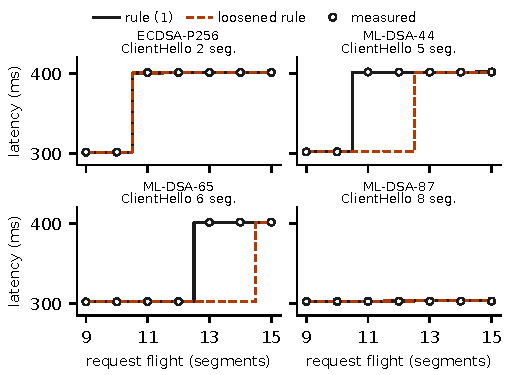
\includegraphics[width=\columnwidth]{fig_stagec_v3}
\caption{Latency of a resumed transaction against the segments of the request flight.}
\label{fig:stagec}
\end{figure}

\emph{The ticket.} That leaves the server's side. The ticket embeds the client certificate (\NstSegMlFourFour\ to \NstSegMlEightSeven\ segments for ML-DSA-44, -65, and -87), and the model had joined it to the response flight. Suppose instead that OpenSSL writes it separately, as soon as the Finished arrives (the early-ticket model, Fig.~\ref{fig:ticket}). If the request flight needs an extra round trip, as with ML-DSA-44, the ticket has been acknowledged by the time the response leaves and no longer occupies the window; if not, as with ML-DSA-65, ticket and response share the window. Independent data, from connections without resumption, agree: the \DubN\ server segment counts of Dubetskyy and Cano~\cite{dubetskyy2026} come out right only if the two NewSessionTicket messages and the close\_notify alert each occupy a segment of their own (our calculation, made after their numbers were published). Deleting the ticket from the model does not work: that fixes ML-DSA-44 but makes the ML-DSA-65 prediction a round trip too short (\CfNoneMlSixFive\ against \CfMeasMlSixFive\ms measured; post hoc, \texttt{counterfactual\_\allowbreak noticket.py}). The early-ticket model reproduces the \RN\ resumed configurations with a mean error of \REarlyMae\ms, but it was developed on them, so this is not a test. The test is a second set of advance predictions (\DN\ cells; requests of 302 and 19\,460 bytes; responses of 3--12 segments), with \DDiff\ discriminating cells for the two ticket models. The early-ticket model is right on all of them and the joined-ticket model on none (exact sign test $p=\SignDP$; Table~\ref{tab:tests}).

\begin{figure}[t]
\centering
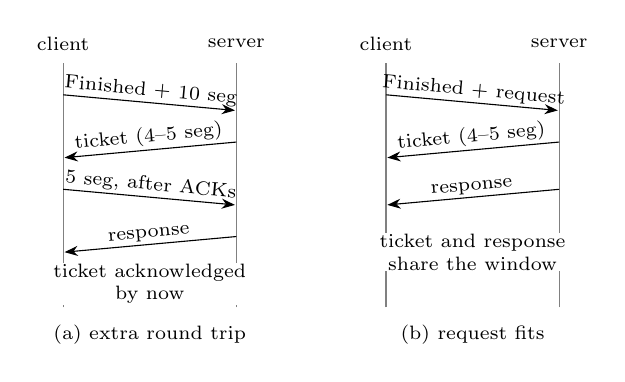
\begin{tikzpicture}[x=1mm,y=1mm,font=\scriptsize,>=Stealth,lab/.style={fill=white,inner sep=0.5pt},a/.style={->,shorten >=0.5pt}]
\foreach \o in {0,41}{\node at (\o,33.5) {client}; \node at (\o+22,33.5) {server}; \draw[gray] (\o,0) -- (\o,31); \draw[gray] (\o+22,0) -- (\o+22,31);}
% (a) the request flight needs an extra round trip
\draw[a] (0,27) -- node[above,sloped,inner sep=1pt] {Finished + 10 seg} (22,25);
\draw[a] (22,21) -- node[above,sloped,inner sep=1pt] {ticket (4--5 seg)} (0,19);
\draw[a] (0,15) -- node[above,sloped,inner sep=1pt] {5 seg, after ACKs} (22,13);
\draw[a] (22,9) -- node[above,sloped,inner sep=1pt] {response} (0,7);
\node[lab,align=center] at (11,3) {ticket acknowledged\\by now};
\node at (11,-3.5) {(a) extra round trip};
% (b) the request fits in the window
\draw[a] (41,27) -- node[above,sloped,inner sep=1pt] {Finished + request} (63,25);
\draw[a] (63,21) -- node[above,sloped,inner sep=1pt] {ticket (4--5 seg)} (41,19);
\draw[a] (63,15) -- node[above,sloped,inner sep=1pt] {response} (41,13);
\node[lab,align=center] at (52,7) {ticket and response\\share the window};
\node at (52,-3.5) {(b) request fits};
\end{tikzpicture}
\caption{Ticket timing: (a) the request flight needs an extra round trip; (b) it does not.}
\label{fig:ticket}
\end{figure}

\section{What Sets the Server's Window after the Ticket}\label{sec:server}
\emph{How large.} Both ticket models fail on the same \DBothWrong\ cells (ML-DSA-44 and -65, a request that needs an extra round trip, responses of 11--12 segments). The latency in these cells implies that the server's window exceeded ten once the ticket had been acknowledged, which neither model allows. A third test (\EN\ cells, responses of 10--18 segments) maps this window. The largest response that avoids an extra round trip is \EFitEcdsa, \EFitMlFourFour\ and \EFitMlSixFive\ segments for tickets of \NstSegEc, \NstSegMlFourFour\ and \NstSegMlSixFive\ segments (ECDSA-P256, ML-DSA-44, and -65). When server and client use different algorithms, this limit follows the client's certificate, and hence the ticket, in \MixRight\ of \MixN\ pairs, a small sample (the exception, server ECDSA-P256 with client ML-DSA-65, reaches \MixFitExc\ instead of \MixPredExc). The limit also depends on the network. In a \GenCells-cell scan (RTT \GenRttLo--\GenRttHi\ms, \GenRateLo--\GenRateHi\,Mbit/s, MTU \GenMtuLo--\GenMtuHi) the largest response without an extra round trip is \GenWMFourFourRttThirty\ and \GenWMSixFiveRttThirty\ segments for ML-DSA-44 and -65 at 30\ms, and \GenWMFourFourMtuLow\ for ML-DSA-44 at MTU~\GenMtuLo\ (ML-DSA-65 shows no step up to the largest response tested, \GenRespMax\ segments). At \GenRttLo\ms RTT and at \GenRateLo\,Mbit/s, by contrast, every suite stays at \GenWEcRttFive. With server-only authentication the ticket fits in one segment, the limit is \ServWindow\ for all three suites, and the early-ticket model, with its window of ten, is wrong on \ServWrong\ of \ServCells\ cells, as predicted before the measurement.

\emph{No ticket, no enlargement.} We predicted, and then measured, what happens when the server issues no ticket on resumed connections: the burst is at most ten segments in all \NtkCells\ cells, including the \NtkEffect\ where it exceeds ten with the ticket (exact sign test on those pairs, $p=\SignNtkP$, the smallest value seven pairs can give).

\emph{One early ACK does not decide it.} At least one ticket segment is acknowledged before the response is written in \RaceBeforePct\% of \RaceN\ captured transactions, many of which keep a window of ten. With all events timed on a single clock, the share is \RqKSixPct\% and \RpKSixPct\% of \RpKSixN\ in two repeats with the CPU clock fixed, and \RuKSixPct\% with the clock left to the system. We then found a better predictor: the burst exceeds ten when the ticket's \emph{last} ACK arrives more than \RaceThr\ms after the last request segment. This timing rule is right on \RaceRight\ of the \RaceMlN\ ML-DSA transactions of the run that produced it, and on \RaceTwoRight\ of \RaceTwoScored\ cells of a request-size sweep predicted beforehand (cells within \RaceBand\ms of the threshold excluded). Without refitting, it classifies \RpKSevenRight--\RqKSevenRight\ of \RoKSevenN\ transactions per run on the X250 and the OptiPlex with the CPU clock fixed. With the clock left to the system, however, the best threshold moves to \RuKSevenBestLo\ms, and on the GX10 the rule misses its criterion (\RgKSevenRight\ of \RgKSevenN; 90\% required). It is a machine-dependent proxy, not a mechanism (supplement).

\emph{Inside the kernel.} Traces show that \texttt{tcp\_slow\_start} runs exactly when the kernel's own test holds (\StPOneRight\ of \StPOneN\ ACKs, as registered). A first burst formula, the window at the time of the write minus the unacknowledged ticket segments, was within one segment in only \StPTwoPct\% of transactions (90\% required). Some ACKs are \emph{late}, that is, processed after the response write has returned, and neither of two registered explanations, socket ownership and the softirq queue, held (rows 10 and 11). We then delayed the client's pure ACKs and read the kernel's counters at each one. After a first round that failed its criteria, a pilot on the GX10 fixed the thresholds and a new burst formula: the smaller of the response and the window left by the last ACK processed before the first ACK of the response can return. In the test on the X250, the window followed the slow-start rule after \RbTestEvOk\ of \RbTestEvN\ window events, and the formula held in \RbTestTxOk\ of \RbTestTxN\ transactions; the delay, however, did not change the order of ACKs and write there (two criteria not met). That the window obeys the kernel's code is expected; the test adds that these counters suffice to determine the burst. We then delayed the server's write instead. That round missed two criteria on the X250; a registered confirmation on new data met all four there, moving the share of late transactions (ML-DSA-87) from \RdXLateZero\% to \RdXLateMax\%, and predicting that share from undelayed transactions and the measured shift of the write (\RdXCellsIn\ of \RdXCellsN\ cells within the band; mean error \RdXMeanErr\ percentage points, against \RdXNullErr\ if the delay is assumed to have no effect). On the GX10 it met two of four, and assuming no effect predicted slightly better. On the i9 it met all four, but weakly: even without delay few transactions are late there (supplement).

\emph{What can be said.} Given when the kernel processes each ACK, the slow-start rule determines the server's window, and the window determines the burst. The size of the ticket decides which ACKs can enlarge that window. With six segments or more, even ACKs processed before the write do, because the socket then counts as cwnd-limited ($10<2\times6$); with fewer, only ACKs processed while the response is in flight do. Unknown are how to predict the processing times from network parameters, why some ACKs are late, why the window grows in some transactions of a cell and not in others (Section~\ref{sec:other}), and why the model misses certain GnuTLS cells.

\begin{table}[t]
\caption{Registered tests and outcomes.}
\label{tab:tests}
\centering\footnotesize\setlength{\tabcolsep}{3pt}
\begin{tabular}{@{}r>{\raggedright\arraybackslash}p{0.57\columnwidth}>{\raggedright\arraybackslash}p{0.31\columnwidth}@{}}
\toprule
 & Test and rule & Result\\
\midrule
1 & Client window: rule~(1) & \CWrongZero\ of \CN\ (met)\\
2 & Client window: loosened by 2 segments & \CWrongTwo\ of \CN\ (refuted)\\
3 & Ticket joined with response, discriminating cells & \DJoinedWrongDiff\ of \DDiff\ (refuted)\\
4 & Ticket written on Finished, discriminating cells & \DEarlyWrongDiff\ of \DDiff\ (met)\\
5 & Ticket written on Finished, all cells & \DEarlyWrong\ of \DN\\
6 & Request-size sweep, ticket-timing rule, cells outside the borderline band & \RaceTwoRight\ of \RaceTwoScored\ (met)\\
7--11 & Processing of the ticket's acknowledgments (kernel trace, state trace, socket backlog, softirq queue; details in the supplement) & trace \KerRight\ of \KerN; state test \StPOneRight\ of \StPOneN\ (met); burst \StPTwoPct\%, backlog \BkAPct\% and \BkBPct\%, softirq \HAPct\% (not met)\\
12 & No ticket issued: response burst of at most 10 segments & \NtkCells\ of \NtkCells\ (met)\\
13 & Rows 1--5 repeated on OpenSSL 4.1.0 and 3.6.5, same machine, 3.5 as baseline (criteria G1--G4) & \GxFourMet\ (4.1.0) and \GxThreeMet\ (3.6.5) of 4 (met)\\
14 & Rows 1--5 and the ticket position on Go \texttt{crypto/tls} (criteria H1--H5) & \GoMet\ of 5 (not met: H1, H5)\\
15 & Window after a short flight under BBR and under fq pacing, plain TCP: X250, i9 (criteria Q1--Q5, seven checks) & X250 \GelevenMet\ of \GelevenN, i9 \GelevenIMet\ of \GelevenIN\ (met)\\
16 & Ticket timing on new cells: RTT 30 and 200\ms, requests of 302--19\,460\,B, OpenSSL~3.5 (criteria K1--K4 per RTT) & \GtwelveMet\ of \GtwelveK\ (met)\\
17 & Client-window and ticket-timing tests under BBR (criteria B1--B5) & \GfBbrMet\ of \GfBbrK\ (met)\\
18 & The same tests with delayed acknowledgments (criteria D1--D5) & \GfDelMet\ of \GfDelK\ (met)\\
19 & Window rule under loss of 0.1, 0.5 and 1\%, plain TCP: X250, i9 (criteria L1--L3) & X250 \GsixMet\ of \GsixK\ (not met: L1); i9 \GsixIMet\ of \GsixIK\ (met)\\
20 & Random held-out test: 100 cells drawn from a stated design space (criteria R1--R5) & \GnineMet\ of \GnineK\ (not met: R1, R3, R5)\\
21 & The three BBR cells of row 17 that deviate, measured again with $n=200$ (criteria S1--S2) & \GtwentyMet\ of \GtwentyK\ (met)\\
22 & Tails of six cells, $n=1\,000$ (criteria T1--T2) & \GtwentyoneMet\ of \GtwentyoneK\ (met)\\
23 & Pipelined variant of the model on 60 new Go cells (criteria P1--P4) & \GeighteenMet\ of \GeighteenK\ (met)\\
24 & Background load, four levels: cross traffic, CPU load, both (criteria Y1--Y4) & \GseventeenMet\ of \GseventeenK\ (met)\\
25 & Physical link, OptiPlex to X250 (criteria F1--F3, and D1--D5 of row 18) & \GthirteenMet\ of \GthirteenK\ (met)\\
26 & The ECDSA-P256 cell of row 20 measured again ($n=200$) and five neighboring cells that test the ticket size of the model (criteria U1--U4) & \GnineBMet\ of \GnineBK\ (met)\\
27 & Rows 7--11 on one clock, CPU clock fixed: X250, OptiPlex, and i9 (K1, K2, K4, K5), GX10 (D1--D5) & X250/OptiPlex 8 of 11 (not met: K1); i9 4 of 4 (met); GX10 3 of 5 (not met: D1, D4)\\
28 & Row 20 on the GX10, OptiPlex, and i9 (criteria A1--A4) & GX10 \GnineRepGxMet\ of \GnineRepGxK, i9 \InineRandMet\ of \InineRandK\ (met); OptiPlex \GnineRepOpMet\ of \GnineRepOpK\ (not met: A2)\\
29 & Rows 16 and 18 on the GX10, OptiPlex, and i9; row 17 on the i9 & \GtwelveRepMet\ of \GtwelveRepK; i9 \InineTktMet\ of \InineTktK\ and \InineBbrMet\ of \InineBbrK\ (met)\\
30 & Rows 1--5 on the GX10 and i9 (criteria G1--G4) & \RoneMet\ of \RoneK\ (met)\\
31 & Server window in the nine random cells where it decides a round trip: X250, GX10, i9 (criteria Q1--Q5; i9 also S1--S3) & X250 \GtfXMet\ of \GtfXK, i9 \GtfIMet\ of \GtfIK\ and S1--S3 (met); GX10 \GtfGxMet\ of \GtfGxK\ (not met: Q5)\\
\bottomrule
\end{tabular}
\end{table}

\section{Does It Replicate?}\label{sec:repl}
We repeated the plain-TCP test (stage~A, four configurations, ten repetitions) on four kernels of the X250 (6.8, 6.14, 6.17, 7.0), on an i9-10900K workstation (7.0.0-42, two runs), and on the GX10 (6.14 and 7.0). In all \NRunsW\ runs rule~(1) is exact in the base, MTU 1\,280 and $w_0=20$ configurations. At MTU~9\,000 only \MtuLo--\MtuHi\% of the flight sizes match on every machine, which points to the jumbo-frame configuration (Section~\ref{sec:window}), not to a particular kernel or CPU. Table~\ref{tab:repl} adds the state test (\texttt{tcp\_\allowbreak slow\_\allowbreak start} runs iff the kernel's window test holds), the no-ticket cells with a burst of at most ten, and the share of ticket ACKs processed from the socket backlog.

Most ticket results carry over from the X250 to the GX10. The state test always holds. Without a ticket the response burst stays within ten segments in all \ArmNoTktCells\ cells; with it, the burst changes in \ArmTktChangeW\ of them on both GX10 kernels and in \NtkEffectW\ on the X250. The two queueing explanations fail again: on the GX10, \ArmBkSixFourteen\% and \ArmBkSevenZero\% of ticket ACKs are processed from the socket backlog (\BkIPct\% on the X250), and only \ArmLateSixFourteen\ of \ArmLateNSixFourteen\ and \ArmLateSevenZero\ of \ArmLateNSevenZero\ are processed after the write returned (\HALate\ of \HN\ on the X250). The first burst formula of Section~\ref{sec:server} meets its criterion on the GX10 (\ArmBurstSixFourteen\% and \ArmBurstSevenZero\%) but not on the X250 (\StPTwoPct\%). The criterion that the \RaceThr\ms timing rule agree with the kernel's state near the threshold fails on both (\ArmThrSixFourteen\% and \ArmThrSevenZero\% on the GX10, \StPThreePct\% on the X250).

\emph{Client window and ticket timing.} The central tests of Section~\ref{sec:ticket} hold on two further machines. Rows 1--5, repeated on the GX10 and the i9 (row 30), met all criteria: rule~(1) was wrong on none of the \CN\ client-window cells, and the early-ticket model on none of the \DDiff\ discriminating cells and, over all \RoneDN\ ticket cells, on \RoneGxEarly\ (GX10) and \RoneIEarly\ (i9). The criteria of rows 16, 17, and 18 were met on the i9 too (row 29).

\emph{A physical link.} We repeated two tests over an Ethernet cable from an OptiPlex client to an X250 server (row 25), both with Linux 7.0.0-42 and Intel e1000e NICs at 1\,Gbit/s, with TSO, GSO, and GRO enabled. \texttt{tc netem} on both NICs emulates the delay. On plain TCP the median window equals rule~(1) at all \GthirteenSizesN\ sizes at RTT 100 and 30\ms, and \GthirteenConnOk\ of \GthirteenConn\ connections (\GthirteenConnPct\%) end with that window (F1--F3 met). On the cells of row 18 ($n=30$, predictions unchanged) rule~(1) is wrong on \GthirteenCWrong\ of \GthirteenCN\ client-window cells, the early-ticket model on \GthirteenEarlyAll\ of \GthirteenDN\ ticket-timing cells and the joined-ticket model on \GthirteenDiscJoined\ of \GthirteenDisc\ discriminating cells (D1--D5 met).

\begin{table}[t]
\caption{Replication on other kernels and CPUs.}
\label{tab:repl}
\centering\footnotesize\setlength{\tabcolsep}{3pt}
\begin{tabular*}{\columnwidth}{@{\extracolsep{\fill}}lcccc@{}}
\toprule
Platform, kernel & MTU 9\,000 & state & no ticket & backlog\\
\midrule
X250, 6.8 / 6.14 / 6.17 & \MtuISixEight\ / \MtuISixFourteen\ / \MtuISixSeventeen\% & -- & -- & --\\
X250, 7.0 & \MtuISevenZero\% & \StPOneRight/\StPOneN & \NtkCells/\NtkCells & \BkIPct\%\\
i9-10900K, 7.0 (2 runs) & \MtuNineI\% & -- & -- & --\\
GX10, 6.14 & \MtuArmSixFourteen\% & \ArmStateSixFourteen/\ArmStateSixFourteen & \ArmNoTktOk/\ArmNoTktCells & \ArmBkSixFourteen\%\\
GX10, 7.0 & \MtuArmSevenZero\% & \ArmStateSevenZero/\ArmStateSevenZero & \ArmNoTktOk/\ArmNoTktCells & \ArmBkSevenZero\%\\
\bottomrule
\end{tabular*}
\end{table}

\section{Other Releases, Libraries, Controllers, and Further Tests}\label{sec:other}
\emph{OpenSSL releases.} The code that writes the ticket is textually identical in 3.5.4, 3.5.9, and 3.6.5, and 4.1.0 keeps the same order of writes. When we repeated the client-window and ticket-timing cells on 3.6.5 and 4.1.0 with a 3.5 baseline (row 13; predictions fixed in advance), both met all four criteria, with the same error counts as 3.5 and latencies within \GxMaxDiff\ms of it.

\emph{A second library.} Go's \texttt{crypto/tls} writes the ticket with the server's first flight and keeps the client's certificates in it, so the sizes and positions of its writes differ from OpenSSL's. With these calibrated on our Go probe and the model otherwise unchanged, we repeated the two tests (row 14, one machine); \GoMet\ of the \GoKW\ registered criteria were met. The variant with the ticket in the first flight was wrong on \GoDisGoWrong\ of the \GoDisN\ discriminating cells and on \GoWrongAll\ of all \GoDN\ ticket cells. Rule~(1) was wrong on \GoCWrong\ of \GoCN\ client-window cells (at most two allowed), and the byte-count check failed until we accounted for a \GoClose-byte \texttt{close\_notify} (supplement).

All \GoWrongSuiteN\ wrong Go cells of the two tests are ML-DSA-87, each a round trip faster than predicted. A packet capture shows why. The server's first flight (\GoChMlEightSeven\ segments) exceeds its window of ten, and the client sends its Finished and request without waiting for the tail of that flight, which holds the end of the ticket. A pipelined variant that no longer waits for the tail, devised after seeing the data, leaves \GoPostAfter\ of the \GoPostBefore\ cells wrong. We then registered the predictions of both models for \GeighteenN\ new ML-DSA-87 cells and \GeighteenCtlN\ ML-DSA-65 controls (row 23). The pipelined variant was wrong on \GeighteenWrongPip\ of the new cells and the original on all \GeighteenWrongGo; all four criteria were met.

\emph{A third library.} GnuTLS~3.8.14 sends two tickets after the client's Finished, each with the client's certificates (\GtlsTicketMinKB\ to \GtlsTicketMaxKB\,KB). On the X250 and the GX10, model unchanged, we varied the number of tickets from zero to four at a fixed suite, client window, and request. Two explanations differ on \GtlsATInflight\ of \GtlsATN\ cells: the tickets share the server's window of ten with the response, as in the model, or they are acknowledged first and enlarge the window by rule~(1). Latency followed the model on all of them: when the request fits in the window, ticket size alone does not set the server's window. The model was wrong on \GtlsADWrong\ of 85 ticket-position cells and \GtlsARWrong\ of 40 random cells on the GX10 (\GtlsXDWrong\ and \GtlsXRWrong\ on the X250), always predicting too long a latency, with \GtlsSharedWrong\ wrong cells common to both machines. The random-cell errors exceed the band of 0--3 set beforehand (supplement).

\emph{Other controllers and pacing.} All \GelevenN\ plain-TCP checks (row 15), hypothesized from the kernel source, were met on the X250 and again on the i9, with the same median windows. Under BBR (the in-tree v1) the window after $n$ segments is $w_0+n$ for every $n$, because BBR adds the acknowledged packets without checking whether the sender was cwnd-limited. Under fq pacing with Reno or Cubic the window still follows (1), except that \GelCubDiffW\ of \GelCubSizes\ sizes differs, by \GelCubDeltaW\ segments (Cubic, $n=\GelCubAt$).

\emph{Ticket tests with BBR and delayed ACKs} (rows 17 and 18, predictions fixed in advance). Under BBR the model with window $w_0+n$ was wrong on \GfBbrCWrong\ of \GfBbrCN\ client-window cells, and rule~(1) on all \GfBbrRuleWrong\ discriminating ones. All \GfBbrK\ criteria were met, though narrowly for the ticket: on \GfMidNW\ ML-DSA-87 cells the latency falls between the BBR and Reno predictions, and one ECDSA cell is \GfLow\ms below both. With delayed ACKs, neither rule~(1) nor the early-ticket model was wrong on any cell, while the joined-ticket model was wrong on \GfDelJoinedDiff\ of \GfDelDDiff\ discriminating cells; all \GfDelK\ criteria were met.

\emph{Ticket timing on new cells.} Support for the early-ticket model rested on \DDiff\ discriminating cells at one RTT, so we tested 30 and 200\ms (row 16; \GtwelveCells\ cells, \GtwelveDis\ discriminating). All \GtwelveK\ criteria were met. The early-ticket model was wrong on \GtwelveEarlyDis\ of the discriminating cells and the joined-ticket model on \GtwelveJoinedDis. Over all cells the early-ticket model was wrong on \GtwelveEarlyAll, the same cell at both RTTs, where it predicts a round trip that did not occur.

\emph{Randomly drawn cells.} We drew \GnineN\ cells at random from a stated design space (suite; request, 302 to 22\,000\,B; response, 222 to 20\,000\,B; RTT, 20 to 200\ms; rate, 10 to 1\,000\,Mbit/s; MTU, 1\,280 to 1\,500; row 20 of Table~\ref{tab:tests}) and fixed the predictions of the early-ticket model before the run. It was right to within half an RTT on \GnineOtherN\ cells, with a mean absolute error of \GnineMaeOther\ms over them, and to within 2\ms on \GnineWithinTwo\ cells. Yet only \GnineMet\ of the \GnineK\ registered criteria were met: the model was wrong on \GnineWrongW\ cells (at most three allowed), the mean absolute error over all \GnineN\ cells was \GnineMae\ms (limit 2), and on the \GnineDisc\ cells that discriminate between the ticket models it was wrong on \GnineDiscEarlyW\ (none allowed). All \GnineWrongW\ errors are predictions one round trip too long, for responses of \GnineRespLo\ to \GnineRespHi\ segments: \GnineLargeWrongW\ of the \GnineLargeN\ cells with a response of 12 segments or more, \GnineMidWrongW\ of \GnineMidN\ with 9 to 11, \GnineSmallWrongW\ of \GnineSmallN\ with fewer (a split made afterwards). We traced the discriminating-cell error to the model's ticket, which is \TktDiffLo\ to \TktDiffHi\ bytes too large; at that MSS this turns one segment into two. With the measured size, the model is right on that cell and on five neighboring cells predicted beforehand (row 26; supplement). Another \GnineOffNW\ cells, all at \GnineOffRate\,Mbit/s, are off by \GnineOffLo\ to \GnineOffHi\ms.

\emph{The window in the remaining wrong cells.} The other \TktWrongAfterW\ wrong cells show the signature of Section~\ref{sec:server}, so we then measured the server's window (row 31) in the nine of the \GnineN\ cells in which a window above ten would save a round trip: the \TktWrongAfterW\ wrong ones and five never wrong, 60 transactions per cell and machine, with the kernel's window read at every ACK. On the X250, GX10, and i9, a transaction was a round trip fast exactly when that window held the whole response in \GtfAgree\ of \GtfW\ transactions with a window reading (post hoc; as registered on the i9, \GtfIAgree\ of \GtfIW). In the \TktWrongAfterW\ unexplained cells, \GtfUFastFit\ of \GtfUFast\ fast transactions had such a window and all \GtfUSlow\ slow ones a smaller one. The client's first request round was never smaller than rule~(1) gives and larger in only \GtfLarger\ of \GtfN\ transactions, so the saving in those cells is not the client's (in one never-wrong cell on the GX10 it was, in five transactions; supplement). The GX10 missed one criterion, a bound on fast transactions that three exceeded because the registered script counted the \texttt{close\_notify} as a response segment. The share of fast transactions in a cell varies between machines and repetitions, and we do not know why.

\emph{Load and tails.} We applied four load levels: none, cross traffic, a busy loop on every CPU, and both (row 24). The model was wrong on \GseventeenWrongMax\ of \GseventeenCells\ cells at every level; load shifted the excess latency of a cell by at most \GseventeenShiftMax\ms, and all four criteria were met. Measured again with $n=200$, the three deviating BBR cells stay within \GtwentyMaxDiff\ms of their first values (row 21). In six cells with $n=\GtwentyoneMinN$ (row 22), the maximum is at most \GtwentyoneMaxMx\ms above the median, so their tails hide no extra round trip.

\section{Recommendations and Limits}\label{sec:recs}
These apply to the tested stack: Linux 7.0, Reno or Cubic, and OpenSSL~3.5 (also 3.6.5 and 4.1.0 in the ticket tests). Under BBR, use $w_0+n$ as the window.
\begin{enumerate}
\item \emph{Budget each direction and each write in segments of the actual MSS.} A flight can cost an extra round trip if it exceeds the window left by the previous flight in the same direction. Compute that window with (1) instead of assuming $w_0$, and count tickets and every other separate write.
\item \emph{Treat the size of the ClientHello as a threshold.} With $w_0=10$, a few extra bytes (a ticket, say) that turn a five-segment ClientHello into a six-segment one raise the window from \WFive\ to \WSix. The next client flight may then fit and save a round trip: a larger ClientHello is not necessarily a costlier one.
\item \emph{After a ticket, budget the response flight at ten segments.} Ticket and response share the window if the request fits; if the request needs an extra round trip, the ticket's ACKs can enlarge the server's window to \SrvWinLo--\SrvWinHi\ segments. Where ten was wrong in Section~\ref{sec:server}, it was pessimistic, and in the \OsRuns\ cell-runs counted in the supplement (OpenSSL with Reno or Cubic; loss, jumbo frames, and BBR excluded), the model never underestimated latency by more than half a round trip.
\item \emph{Measure the server's window on the actual path.} After a ticket, the window depends on which ACKs the kernel processes while the sender counts as cwnd-limited, and therefore on RTT, rate, MTU, and processing times. No rule here predicts it from the network.
\item \emph{Before relying on (1), check it on your kernel, and check how your TLS library writes.} With jumbo frames, also make sure that the receive buffer can hold the flight; otherwise the sender is not cwnd-limited and (1) does not apply.
\end{enumerate}

\emph{Limits: scope.} The window rule was tested on \NCombW\ machine-kernel combinations (\NRunsW\ runs). The kernel tests of Table~\ref{tab:repl} ran on two machines; rows 1--5 on three; rows 16 and 18 on four; row 20 on four; row 31 and the last intervention round on three; rows 15, 17, and 19, the GnuTLS tests, and the earlier intervention rounds on two; the Go, load, and release tests on one; and row 25 on a pair. All delay is emulated, even over the cable; no Internet path was used. Loss was tested on plain TCP only, RTT variation not at all, and background load with a single traffic mix. Each measurement used one connection, so concurrency, CPU cost, and throughput are untested; BBR pacing is not modeled. Transactions use mutual authentication (except the server-only cells of Section~\ref{sec:server}), usually with \NPerCell\ per cell, and Reno or Cubic unless stated. Most wrong cells of the random draw (\DomLargeWrong\ of \DomWrongTotal\ cell-runs over five runs) and all wrong GnuTLS cells have a request over 13\,KB (supplement), and which cells fail depends partly on the machine (row 28). Full handshakes are not evaluated.\par\emph{Limits: the TLS library.} We measured OpenSSL (three releases that share the ticket-writing code), Go's \texttt{crypto/tls} on one machine, and GnuTLS on two. The window rule and ACK processing are Linux's; a ticket's timing and size are the library's: OpenSSL and GnuTLS write it after the client's Finished, Go with the server's first flight, and wolfSSL 5.9.4 (source inspected, not measured) keeps no ML-DSA certificate in its ticket.

\section{Conclusion}
A few bytes can decide a round trip. From an initial window of ten, a five-segment flight leaves the window where it was and a six-segment flight raises it by two, because in slow start Linux grows the window only while the sender counts as cwnd-limited (RQ1). Our model had gone wrong on the server's side: OpenSSL writes the session ticket separately, so the response either shares the window with it or finds it already acknowledged (RQ2). The ticket's ACKs can then enlarge the server's window by several segments, following the slow-start rule at whatever times the kernel processes them (RQ3).

Practitioners can budget Reno and Cubic flights with (1) and our recommendations; in our counted tests, the model behind them erred by more than half a round trip only by predicting too long a latency. Still, measure the response flight on the actual path. What remains open is why the kernel processes the ACKs when it does.

\emph{Acknowledgments.} The first author used ChatGPT (OpenAI) and Claude (Anthropic) for analysis scripting, language editing and consistency checks; both authors reviewed and edited the code and the text and take full responsibility for it.
\par\emph{Availability.} Scripts, data, the pre-registered predictions (with commit times) and derived tables are on Zenodo: doi:\allowbreak10.5281/\allowbreak zenodo.\allowbreak24355942 (all versions) and doi:\allowbreak10.5281/\allowbreak zenodo.\allowbreak24417627 (version l1-v1.3). Raw traces: doi:\allowbreak10.5281/\allowbreak zenodo.\allowbreak24384873 and doi:\allowbreak10.5281/\allowbreak zenodo.\allowbreak24419058; the traces of November 25 and 26: \pending{DOI}. Appendix~\ref{app:repl} says how to repeat the key results.

\appendix
\section{Repeating the Key Results}\label{app:repl}
The archive (Availability) holds the code, the predictions fixed before each measurement, the derived data, and the analysis outputs. Its layout is that of our working repository, and the paths below are relative to it. Results can be repeated at three levels.

\emph{Level 1: numbers and figures (minutes, no root).} With Python~3, the packages in \texttt{requirements.txt}, and \TeX\ Live, \texttt{bash reproduce\_\allowbreak l1.sh} regenerates the figures and the generated numbers from the shipped data and analysis outputs, compares them with the shipped copies, reruns the kernel-logic program of Section~\ref{sec:window} and the analyses whose data files are shipped, and builds the paper and the supplement. It stops at the first difference. The last table of the supplement names the script and output behind each number.

\emph{Level 2: analyses from raw traces.} The packet captures and kernel traces are separate records (Availability). For the ticket ACK tests of rows 6--11, \texttt{bash tools/raw\_traces.sh verify DIR} reruns the analyses on the unpacked traces in \texttt{DIR} and compares the results with the archived outputs. For row~31, run \texttt{analyze\_g24.py} and then \texttt{analyze\_g24\_posthoc.py} (in \texttt{Measurements/testbed/}) on one machine's unpacked traces.

\emph{Level 3: new measurements.} They need a Linux machine with root access, \texttt{tc netem}, and, for kernel traces, \texttt{bpftrace}. In \texttt{Measurements/testbed/}, \texttt{./setup\_host.sh} builds OpenSSL~3.5 and the probes and generates test certificates (we distribute no private keys). The scenario scripts check that the prediction files are committed; in an unpacked archive, first run \texttt{git init} and commit the files. Unless the runner does it, fix the CPU clock with \texttt{sudo ./host\_tune.sh on}. Table~\ref{tab:key} gives the four key results. Absolute latencies and the shares that depend on processing order differ between machines; the outcomes listed are the ones that held on ours.

\begin{table}[t]
\caption{Repeating the four key results (\texttt{.../} stands for \texttt{Measurements/scenarios/shared/}).}
\label{tab:key}
\centering\footnotesize\setlength{\tabcolsep}{3pt}
\begin{tabular}{@{}>{\raggedright\arraybackslash}p{0.22\columnwidth}>{\raggedright\arraybackslash}p{0.40\columnwidth}>{\raggedright\arraybackslash}p{0.32\columnwidth}@{}}
\toprule
Result & Run, then analyze & What should hold\\
\midrule
Window rule~(1), plain TCP (Section~\ref{sec:window}) & \texttt{.../G11\_cc\_\allowbreak pacing/\allowbreak run.sh} (about 10 minutes), which also runs \texttt{analyze\_g11.py} & With Reno and no pacing, rule (1) at 18 or more of 20 flight sizes; under BBR, $w_0+n$\\
Client window and ticket timing (rows 1--5) & \texttt{.../G9\_ticket\_\allowbreak versions/\allowbreak run.sh} (about 75 minutes); \texttt{analyze\_g9.py --run 3.5=DIR} & Criteria G1--G4\\
Random cells (row 20) & \texttt{.../G19\_random\_\allowbreak design/\allowbreak run.sh} (about an hour), which also runs \texttt{analyze\_g19.py} & Almost all cells right; each wrong cell predicted one RTT too long. How many fail varies\\
Server window (row 31) & \texttt{sudo env PQC\_CERTS=\allowbreak\$PWD/../certs bash run\_g24.sh run} (about 15 minutes); \texttt{analyze\_g24.py}, \texttt{analyze\_g24\_posthoc.py} & A fast transaction has a window at least as large as the response; how often one is fast varies\\
\bottomrule
\end{tabular}
\end{table}

\bibliographystyle{ACM-Reference-Format}
\bibliography{refs}
\end{document}
